%xelatex -shell-escape -output-directory=bin ergasia.tex
\documentclass{assignment}

\usepackage{enumitem}


\university{Πανεπιστήμιο Πειραιώς}{Πα.Πει.}
\school{Τμήμα Πληροφορικής}{Π.Μ.Σ. "Πληροφορική"}
\department{Πρόγραμμα Μεταπτυχιακών Σπουδών «Πληροφορική»}{}
%\cover{images/cover.jpg}{http://www.cyberciti.biz/faq/grub-boot-into-single-user-mode/}

\title{Αλληλεπίδραση Ανθρώπου Υπολογιστή \\ Ηλεκτρονικό θεματικό πάρκο σε μεσαιωνική καστροπολιτεία}
%\projectlevel{Εργαστήριο Λειτουργικά Συστήματα}
%\lesson{Λειτουργικά Συστήματα}{1}
\date{Αθήνα, 2014}

\author{Αναγνωστόπουλος Βασίλης - Θάνος, Κατσής Γεώργιος}
%\register{ΜΠΠΛ13002}{1}

%\exercauthor{Αναγνωστόπουλος Βασίλης - Θάνος}{06107083}{9}

%\advisor{Τσακίρη Μαρία, Αναπληρώτρια Καθηγήτρια Ε.Μ.Π.}

\begin{document}

\maketitle
% Να σκεφτώ τί αλλαγές θέλω να κάνω με τις αριθμήσεις και άμα θέλω να κάνω.
% Να σκεφτώ να τις ενσωματώσω και στο assignment.cls

\setcounter{page}{1} 
\pagenumbering{roman}

\pagestyle{plain}
\tableofcontents
\newpage


%\pagestyle{headings}
\pagestyle{fancy}
\setcounter{page}{1} 
\pagenumbering{arabic}

\section{Ανάλυση απαιτήσεων}

Θα πρέπει να δημιουργηθεί ένα σύστημα διεπαφής για τους χρήστες ενός θεματικού πάρκου μιας μεσαιωνικής καστροπολιτείας, η οποία θα αξιοποιηθεί τουριστικά με την προσθήκη ηλεκτρονικών αυτοματισμών, με σκοπό την προσέλκυση τουρισμού.

Στην μεσαιωνική καστροπολιτεία, θα διατίθενται ανεξάρτητα μεσαιωνικά διαμερίσματα, καθένα από τα οποία θα περιβάλλεται από μία τάφρο. Το κάθε διαμέρισμα θα έχει μία πόρτα που θα ανεβαίνει και θα κατεβαίνει και θα λειτουργεί ως γέφυρα πάνω στην τάφρο. Η τάφρος δεν θα υπάρχει μόνο για λόγους ασφάλειας αλλά και για να δημιουργεί ατμόσφαιρα διασκέδασης οπότε θα λειτουργεί επίσης ως ιδιωτική πισίνα για κάθε μεσαιωνικό διαμέρισμα.

Επίσης, στην καστροπολιτεία, θα λειτουργεί καφετέρια-εστιατόριο και σε αυτό το πλαίσιο, οι λειτουργίες κάποιων μηχανημάτων μπορούν να γίνονται ηλεκτρονικά. Θα περιλαμβάνονται κάποιες εικονικές διεπαφές με τους χρήστες για τομείς που δεν είναι ανάγκη να είναι υλοποιήσιμοι (όμως για τον χρήστη θα είναι λειτουργικοί, π.χ. ο χρήστης θα μπορεί να πληρώσει με πιστωτική κάρτα, απλά όπως είναι κατανοητό δεν θα είναι αληθινή η συναλλαγή).  

Συγκεκριμένα ζητούνται τα παρακάτω:

\begin{itemize}
\item Η λειτουργικότητα της εφαρμογής.
\item Τα συνοδευτικά εγχειρίδια τα οποία θα επεξηγούν την εφαρμογή.
\end{itemize}

\subsection{Ανάλυση χρηστών}

Στην αλληλεπίδραση ανθρώπου υπολογιστή λαμβάνουν μέρος δύο πλευρές: ο άνθρωπος και ο υπολογιστής. Ο άνθρωπος, δηλαδή ο χρήστης είναι εκείνος στον οποίο απευθύνεται το οποιοδήποτε σύστημα διεπαφής μεταξύ χρήστη και υπολογιστή. Επομένως το σύστημα διεπαφής πρέπει να σχεδιάζεται έχοντας υπόψη τις ικανότητες και της αδυναμίες του χρήστη της εφαρμογής. Στο σχεδιασμό των εφαρμογών, η ανάλυση των χρηστών είναι η διαδικασία με την οποία οι κατασκευαστές της εφαρμογής καθορίζουν τα χαρακτηριστικά των χρηστών που θα χρησιμοποιούν την εφαρμογή και θα επηρεάσουν την ανάπτυξη της εφαρμογής \cite{wiki:user_analysis,class_notes}.

Ο προσδιορισμός των δυνητικών χρηστών του συστήματος και τα χαρακτηριστικά τους είναι αναγκαία προκειμένου να διασφαλιστεί ότι η εν λόγω εφαρμογή θα είναι πιο φιλική προς τους χρήστες \cite{wiki:user_analysis}.

Στην περίπτωση του συστήματος διεπαφής για τους χρήστες του θεματικού πάρκου της μεσαιωνικής καστροπολιτείας, οι χρήστες της εφαρμογής είναι οι πελάτες της καστροπολιτείας. Επομένως δεν πρέπει να γίνει καμιά παραδοχή για τους χρήστες αυτούς και πρέπει να γίνει πρόβλεψη για όλες τις ηλικίες καθώς και για διαφορετικά επίπεδα εξοικείωσης με την τεχνολογία. 

\subsection{Λειτουργικότητα της εφαρμογής}
%Requirements documentation

Για την επίτευξη της λειτουργικότητας της εφαρμογής θα θεωρήσουμε ότι οι χρήστες της εφαρμογής αποτελούνται από τους πελάτες-τουρίστες της μεσαιωνικής καστροπολιτείας. Επίσης την εφαρμογή θα την χρησιμοποιούν και οι υπάλληλοι της μεσαιωνικής καστροπολιτείας.


Οι χρήστες μέσω της εφαρμογής θα μπορούν να κάνουν τα εξής:

\begin {description}

\item[Αλληλεπίδραση με τις διάφορες συσκευές της καστροπολιτείας:] Γι` αυτό το σκοπό θα δημιουργηθεί ένα σύστημα διεπαφής για την διαχείριση-χειρισμό (από τους πελάτες ή τους υπαλλήλους) των διαφόρων συσκευών (ηλεκτρικών και άλλων) του κάθε μεσαιωνικού διαμερίσματος. Μέσω αυτού του συστήματος οι χρήστες θα μπορούν:

  \begin{itemize}
  \item Να ανάβουν/σβήνουν τα φώτα του μεσαιωνικού τους διαμερίσματος.
  \item Να ρυθμίζουν την θέρμανση/ψύξη του μεσαιωνικού τους διαμερίσματος.
  \item Να ανοίγουν/κλείνουν την τηλεόραση/ραδιόφωνο καθώς και να ρυθμίζουν τα κανάλια.
  \end{itemize}

\item[Διαχείριση της τάφρου-πισίνας:] Γι` αυτό το σκοπό θα δημιουργηθεί ένα σύστημα διεπαφής για τους χρήστες μέσω του οποίου θα μπορούν να ανοίγουν/κλείνουν την γέφυρα πάνω στην τάφρο-πισίνα. Ακόμα θα είναι δυνατόν οι χρήστες να ρυθμίζουν την στάθμη του νερού μέσα στην τάφρο-πισίνα, ενώ ταυτόχρονα θα υπάρχει ένας αισθητήρας που θα ενεργοποιείται/απενεργοποιείται και θα ειδοποιεί τον χρήστη εάν υπάρχουν άνθρωποι μέσα στην πισίνα. Επίσης, θα υπάρχει αισθητήρας που θα ενεργοποιείται ή θα απενεργοποιείται και θα ειδοποιεί τον χρήστη εάν υπάρχουν άνθρωποι μέσα στην πισίνα. Θα υπάρχει η δυνατότητα να ενεργοποιείται συναγερμός από αυτόν τον αισθητήρα ανάλογα την περίπτωση (π.χ. είναι βράδυ και ο ένοικος θέλει να υπάρχει συναγερμός για λόγους ασφαλείας, ή είναι μέρα και ο ένοικος δεν θέλει το συναγερμό λόγω του ότι η τάφρος λειτουργεί ως πισίνα).

\item[Ηλεκτρονικές παραγγελίες:] Θα είναι δυνατόν να δίνονται παραγγελίες από τους πελάτες με σκοπό την εξυπηρέτηση τους, καθώς και ερωτήσεις/αποκρίσεις από τους υπαλλήλους της καστροπολιτείας για την εκκίνηση της παραγγελίας, την πραγματοποίηση και την ολοκλήρωση της. Αυτές οι παραγγελίες μπορεί να αφορούν καφέ ή/ και κάποιο γεύμα ή/και κάποιο ποτό, ανάλογα με την ώρα της ημέρας. Γι` αυτό το σκοπό θα δημιουργηθεί ένα σύστημα διεπαφής για την αλληλεπίδραση πελατών/υπαλλήλων που θα βοηθάει την διαδικασίας παραγγελίας, την εκτέλεση της και την εξόφληση της ή την ενσωμάτωση του λογαριασμού στο γενικό λογαριασμό του πελάτη. Ο υπάλληλος θα φαίνεται στο σύστημα διεπαφής ως εικόνα ενός ιππότη ή μιας πριγκίπισσας. 

\end{description}

\emph{Τί άλλο να βάλουμε από τα Μοντέλα των χρηστών στο σχεδιασμό και τί άλλο να λάβουμε υπόψιν μας ;;;}

Αυτές οι ενέργειες μπορούν να διαιρεθούν σε περισσότερα στάδια. Στο μοντέλο του Norman τα στάδια είναι τα εξής \cite{class_notes}:
\begin{itemize}
\item Θέση του στόχου.
\item Καθορισμός της πρόθεσης.
\item Καθορισμός της σειράς ενεργειών.
\item Εκτέλεση της ενέργειας.
\item Αντίληψη της κατάστασης του συστήματος.
\item Ερμηνεία της κατάστασης του συστήματος.
\item Αξιολόγηση της κατάστασης του συστήματος σε σχέση με τους στόχους και τις προθέσεις.
\end{itemize}

Οι ανάλυση των ενεργειών αυτών γίνεται στην επόμενη ενότητα με την ιεραρχική ανάλυση εργασιών. 

Τέλος ο σχεδιασμός του συστήματος διεπαφής θα γίνει με έναν τρόπο τέτοιο ώστε να έρχεται όσο πιο κοντά στο θέμα της μεσαιωνικής καστροπολιτείας. Γι` αυτό το σκοπό θα περιέχονται στοιχεία όπως κατάλληλη διακόσμηση, πολεμίστρες, μπουντρούμια, κήπους με δέντρα στον εξωτερικό χώρο πριν μπούμε μέσα στο μεσαιωνικό διαμέρισμα, κιάλα, παράθυρα με θέα στην τάφρο κ.λ.π. 

\subsection{Ιεραρχική ανάλυση εργασιών}

Η ανάλυση εργασιών είναι η επεξεργασία της ανάλυσης του τρόπου που οι άνθρωποι κάνουν κάποιες δουλειές και περιλαμβάνει μία λεπτομερή περιγραφή των χειρωνακτικών και πνευματικών εργασιών, την διάρκεια, την συχνότητα και την πολυπλοκότητα των εργασιών και γενικά όλες τους παράγοντες που απαιτούνται από τον χρήστη για την ολοκλήρωση της εργασίας \cite{class_notes,wiki:task_analysis}.

Σε αυτή την ενότητα θα αναλυθούν όλες οι εργασίες που θα μπορούν να πραγματοποιηθούν από τους χρήστες της μεσαιωνικής καστροπολιτείας.

\subsubsection{Άνοιγμα/σβήσιμο φώτων}

Η εργασία "Άνοιγμα/σβήσιμο φώτων" μπορεί να αναλυθεί ως εξής:

\begin{enumerate}
\setcounter{enumi}{-1}
\item Άνοιγμα/σβήσιμο φώτων
\item Ρύθμιση της έντασης των φώτων
\item Ενεργοποίηση των φώτων
\end{enumerate}

Συνοπτικά η ιεραρχική ανάλυση εργασιών για την ρύθμιση των φώτων φαίνεται και στο σχήμα \ref{fig:task_analysis:fota}.

\begin{figure}
\begin{center}
\resizebox*{10.5cm}{!}{
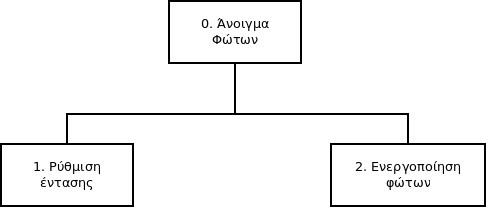
\includegraphics{images/fota.png}}
\caption{Η ιεραρχική ανάλυση εργασιών για την ρύθμιση των φώτων.}
\label{fig:task_analysis:fota}
\end{center}
\end{figure}


\subsubsection{Θέρμανση/ψύξη διαμερίσματος}

Η εργασία "Θέρμανση/ψύξη διαμερίσματος" μπορεί να αναλυθεί ως εξής:

\begin{enumerate}
\setcounter{enumi}{-1}
\item Θέρμανση/ψύξη διαμερίσματος
\item Ρύθμιση της θερμοκρασίας
\item Αλλαγή της θερμοκρασίας
\end{enumerate}

Συνοπτικά η ιεραρχική ανάλυση εργασιών για την ρύθμιση της θερμοκρασίας του διαμερίσματος φαίνεται και στο σχήμα \ref{fig:task_analysis:thermansi}.

\begin{figure}
\begin{center}
\resizebox*{10.5cm}{!}{
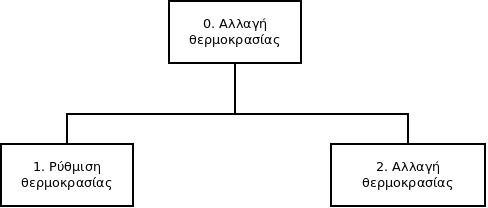
\includegraphics{images/thermansi.png}}
\caption{Η ιεραρχική ανάλυση εργασιών για την ρύθμιση των φώτων.}
\label{fig:task_analysis:thermansi}
\end{center}
\end{figure}

\subsubsection{Ρύθμιση τηλεόρασης/ραδιοφώνου}

Η εργασία "Ρύθμιση τηλεόρασης/ραδιοφώνου" μπορεί να αναλυθεί ως εξής:

\begin{enumerate}
\setcounter{enumi}{-1}
\item Ρύθμιση τηλεόρασης/ραδιοφώνου
\item Επιλογή σταθμού
\item Αλλαγή σταθμού
\end{enumerate}

Συνοπτικά η ιεραρχική ανάλυση εργασιών για την τηλεόρασης/ραδιοφώνου φαίνεται και στο σχήμα \ref{fig:task_analysis:tv}.

\begin{figure}
\begin{center}
\resizebox*{10.5cm}{!}{
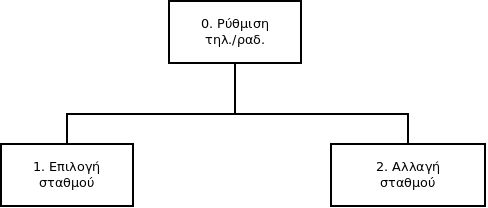
\includegraphics{images/tv.png}}
\caption{Η ιεραρχική ανάλυση εργασιών για την ρύθμιση των φώτων.}
\label{fig:task_analysis:tv}
\end{center}
\end{figure}

\subsubsection{Πραγματοποίηση μίας παραγγελίας}

Η εργασία "Πραγματοποίηση μίας παραγγελίας" μπορεί να αναλυθεί ως εξής:

\begin{enumerate}
\setcounter{enumi}{-1}
\item Παραγγελία μίας παραγγελίας
\item Επιλογή των αντικειμένων που θέλουμε να παραγγείλουμε
  \begin{enumerate}[label*=\arabic*.]
  \item Επιλογή κατηγορίας (π.χ. σαλάτες, ποτό, κ.λ.π.)
  \item Επιλογή αντικειμένων (ανάλογα με την κατηγορία που έχουμε επιλέξει πριν θα φαίνονται και τα αντίστοιχα προϊόντα)
  \item Εμφάνιση λεπτομερειών (μετά την επιλογή του αντικειμένου θα φαίνονται οι λεπτομέρειες για το αντικείμενο αυτό)
  \item Προσθήκη του αντικειμένου στην παραγγελία ή ακύρωση της παραγγελίας
  \item Επιστροφή στην αρχική σελίδα επιλογής κατηγορίας
  \end{enumerate}
\item Ολοκλήρωση της παραγγελίας και εμφάνιση του ολικού ποσού. Εδώ θα δίνεται στον χρήστη αν θα θέλει να ακυρώσει την παραγγελία του ή να συνεχίσει
\item Ετοιμασία της παραγγελίας του χρήστη
\item Αποστολή της παραγγελίας του χρήστη
\item Πληρωμή της παραγγελίας
  \begin{enumerate}[label*=\arabic*.]
  \item Επιλογή του τρόπου πληρωμής (π.χ. πιστωτική κάρτα, μετρητά ή με πίστωση στον λογαριασμού του πελάτη
  \item Ολοκλήρωση της πληρωμής
  \end{enumerate}
\end{enumerate}

Συνοπτικά η ιεραρχική ανάλυση εργασιών για την πραγματοποίηση μίας παραγγελίας φαίνεται και στο σχήμα \ref{fig:task_analysis:paraggelia}.

\begin{figure}
\begin{center}
\resizebox*{16.5cm}{!}{
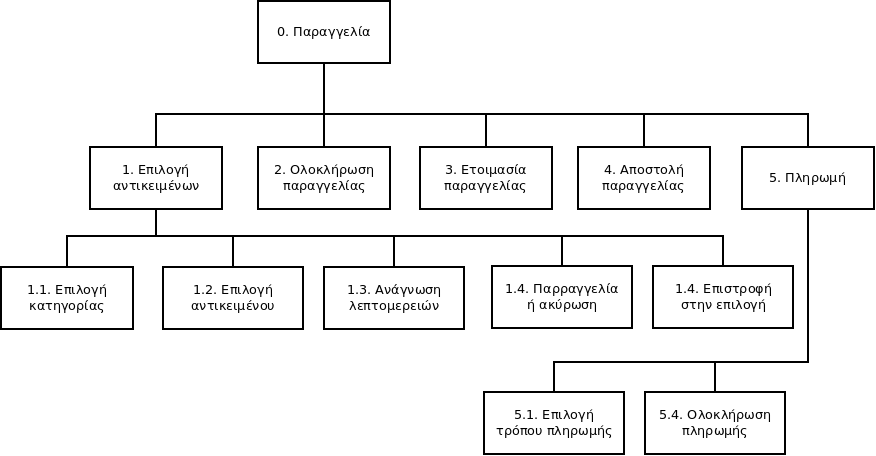
\includegraphics{images/paraggelia.png}}
\caption{Η ιεραρχική ανάλυση εργασιών για την πραγματοποίηση μίας παραγγελίας.}
\label{fig:task_analysis:paraggelia}
\end{center}
\end{figure}

\subsubsection{Ρύθμιση της πισίνας-τάφρου}

Η εργασία "Ρύθμιση της πισίνας-τάφρου" μπορεί να αναλυθεί ως εξής:

\begin{enumerate}
\setcounter{enumi}{-1}
\item Ρύθμιση της πισίνας-τάφρου
\item Έλεγχος για άνρθωπο
  \begin{enumerate}[label*=\arabic*.]
  \item Αν υπάρχει άνθρωπος μέσα στην πισίνα τότε ελέγχουμε και την ώρα
  \item Αν και οι δύο παραπάνω συνθήκες ισχύουν τότε ενεργοποιείται ο συναγερμός 
  \end{enumerate}
\item Ρύθμιση της στάθμης της πισίνας
  \begin{enumerate}[label*=\arabic*.]
  \item Επιλογή της στάθμης από τον χρήστη
  \item Αλλαγή της στάθμης της πισίνας
  \end{enumerate}
\item Ρύθμιση της θερμοκρασίας της πισίνας
  \begin{enumerate}[label*=\arabic*.]
  \item Επιλογή της θερμοκρασίας από τον χρήστη
  \item Έλεγχος της θερμοκρασίας ότι δεν υπερβαίνει κάποια όρια
  \item Αλλαγή της θερμοκρασίας της πισίνας
  \end{enumerate}
\end{enumerate}

Συνοπτικά η ιεραρχική ανάλυση εργασιών για την πραγματοποίηση μίας παραγγελίας φαίνεται και στο σχήμα \ref{fig:task_analysis:pisina}.

\begin{figure}
\begin{center}
\resizebox*{10.5cm}{!}{
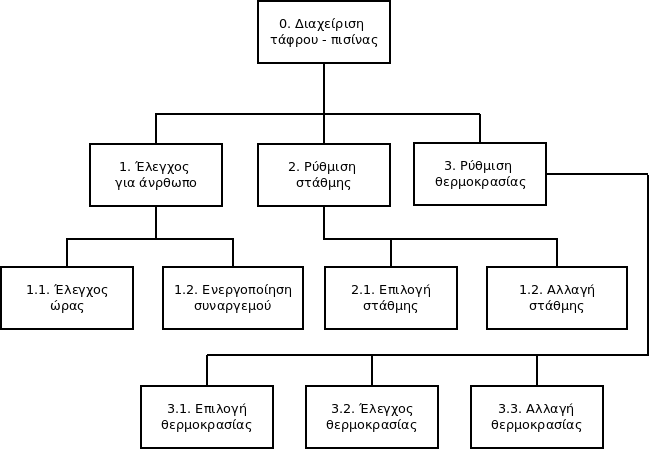
\includegraphics{images/pisina.png}}
\caption{Η ιεραρχική ανάλυση εργασιών για το την ρύθμιση της πισίνας-τάφρου.}
\label{fig:task_analysis:pisina}
\end{center}
\end{figure}

\subsubsection{Άνοιγμα πόρτας της πισίνας-τάφρου}

Η εργασία "Άνοιγμα πόρτας της πισίνας-τάφρου" μπορεί να αναλυθεί ως εξής:

\begin{enumerate}
\setcounter{enumi}{-1}
\item Άνοιγμα πόρτας της πισίνας-τάφρου
\item Έλεγχος για άνρθωπο
\item Άνοιγμα ή κλείσιμο της πόρτας
\end{enumerate}

Συνοπτικά η ιεραρχική ανάλυση εργασιών για την πραγματοποίηση μίας παραγγελίας φαίνεται και στο σχήμα \ref{fig:task_analysis:porta}.

\begin{figure}
\begin{center}
\resizebox*{10.5cm}{!}{
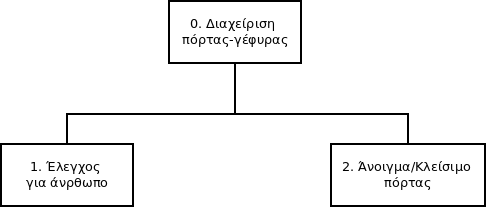
\includegraphics{images/porta.png}}
\caption{Η ιεραρχική ανάλυση εργασιών για το άνοιγμα της πόρτας της πισίνας-τάφρου.}
\label{fig:task_analysis:porta}
\end{center}
\end{figure}

\subsection{Τί αλλο να μπει στο πρωτο κεφάλαιο;;;}
και τί διορθώσεις να κάνω.

\section{Σχεδιασμός}

Σε αυτή την ενότητα θα αναλυθούν οι αποφάσεις που πάρθηκαν κατά την διάρκεια του σχεδιασμού της διεπαφής της καστροπολιτείας

\subsection{Στόχοι}
Οι άμεσοι στόχοι του συστήματος διεπαφής είναι \cite{class_notes}:
\begin{description}
\item [Η μέγιστη δυνατή χρησιμοποιησιμότητα (\en{maximum usability)}]
\item [να είναι φιλικό προς τον χρήστη:] Το σύστημα διεπαφής δεν πρέπει να απωθεί τον χρήστη. Αντίθετα πρέπει να τον ενθαρρύνει να ανακαλύπτει όλες τις δυνατότητες του προγράμματος.
\item [συνεπές:] Τα χρώματα και οι λέξεις πρέπει πάντα να σημαίνουν τα ίδια πράγματα κάθε φορά.
\item [όχι υπερβολικό:] Δεν πρέπει να χρησιμοποιούνται τα χρώματα και τα εικονίδια σε υπερβολή έτσι ώστε να μπερδεύουν το χρήστη αντί να τον διευκολύνουν.
\item [να δοκιμάζεται όσο νωρίτερα γίνεται:] Έτσι ώστε να είναι βέβαιο ότι επιτυγχάνει το στόχο του.
\item [να αποφεύγονται τα λάθη των χρηστών:] Όσο φιλικό και να είναι το σύστημα διεπαφής, ο χρήστης θα κάνει λάθη και θα προσπαθήσει να κάνει πράγματα που δεν γίνονται μέσα στο πρόγραμμα. Επομένως τα πιθανά λάθη των χρηστών θέτουν τους εξής σχεδιαστικούς στόχους:
  \begin{itemize}
  \item Το σύστημα να είναι ικανό να μην χαλάει την λειτουργία του από τα πιθανά λάθη.
  \item Να γνωστοποιείται στον χρήστη τί δεν μπορεί να κάνει.
  \item Να περιορίζεται η πιθανότητα λάθους.
  \item Να προσφέρεται βοήθεια αν ο χρήστης κάνει κάτι λάθος χωρίς όμως να δημιουργείται σύγχυση στο χρήστη από υπερβολικό αριθμό οδηγιών. 
  \end{itemize} 
Η αποφυγή των λαθών επιτυγχάνεται σε μεγαλύτερο βαθμό με τις ακόλουθες βελτιώσεις:
  \begin{itemize}
  \item Τα μηνύματα λάθους να είναι συγκεκριμένα και περιεκτικά.
  \item Να απενεργοποιούνται εντολές που δεν μπορούν να χρησιμοποιηθούν σε μία συγκεκριμένη περίσταση.
  \item Να ολοκληρώνονται αυτόματα κάποιες εντολές όταν έχει δοθεί αρκετή πληροφορία.
  \end{itemize}
\end{description}

Η επιλογή του είδους του συστήματος διεπαφής μπορεί να έχει τεράστια επιρροή στους στόχους του συστήματος διεπαφής. Μερικά συνηθισμένα είδη συστημάτων διεπαφής είναι \cite{class_notes}:

\begin{itemize}
\item Άμεση διαχείριση
\item Σύστημα διεπαφής με γραμμές εντολών (\en{command line})
\item Μενού (\en{menus})
\item Φυσική γλώσσα (\en{Natural language})
\item Ερώτηση/απάντηση (\en{query})
\item Φόρμες και λογιστικά φύλλα
\end{itemize}

Για την επίτευξη των παραπάνω στόχων που τέθηκαν στην αρχή της ενότητας θεωρείται ότι επιτυγχάνονται πιο ολοκληρωμένα με την άμεση διαχείριση. Οι ενέργειες που μπορεί να πραγματοποιήσει ο χρήστης αναπαρίστανται οπτικά και σε αυτή την περίπτωση ο χρήστης διευκολύνεται γιατί μπορεί να χειριστεί οικία πράγματα και να δει αμέσως τα αποτελέσματα \cite{class_notes}. Παρόλα αυτά υπάρχουν και μερικά προβλήματα \cite{class_notes}:

\begin{itemize}
\item Οι οπτικές αναπαραστάσεις δεν είναι απαραίτητα καλύτερες από άλλους τρόπους αλληλεπίδρασης γιατί μπορεί να καταναλώνουν πολύ χώρο και πολλές εντολές μπορεί να απλώνονται σε άλλες σελίδες.
\item Τα εικονίδια που χρησιμοποιούνται μπορεί να μην είναι ιδιαίτερα κατανοητά στο χρήστη.
\item Η οπτική αναπαράσταση μπορεί να είναι παραπλανητική.
\end{itemize}

Για την αντιμετώπιση της πρώτης δυσκολίας θα προτιμηθεί η "συμπύκνωση" των μενού έτσι ώστε να χωράνε σε μία ολόκληρη σελίδα ενώ για της άλλες δύο δυσκολίες (εκτός της προφανής λύσης που είναι να χρησιμοποιηθούν όσο πιο αντιπροσωπευτικά εικονίδια) οι επιλογές της εφαρμογής θα τεκμηριωθούν εκτενώς στα εγχειρίδια που θα παραδοθούν στους τελικούς χρήστες.

Οι υπόλοιπες επιλογές απορρίφθηκαν διότι δεν ήταν αρκετά διαισθητικές και ο χρήστης θα έπρεπε να αφιερώσει αρκετό χρόνο για την εξοικείωση και την εκμάθηση της εφαρμογής.

\subsection{Τί άλλο θεωρητικό να βάλουμε για να δικαιολογήσουμε τις αποφάσεις μας;;;}

\subsection{Παρουσίαση γραφικού περιβάλλοντος}

Σε αυτή την ενότητα παρουσιάζονται οι οθόνες του γραφικού περιβάλλοντος για την επίτευξη της λειτουργικότητας της εφαρμογής.
\emph{Εδώ να βάλουμε την λογική πίσω από την κάθε οθόνη της εφαρμογής και πως λειτουργεί.}\\

\subsubsection{Γενικό Μενού - Εισαγωγική οθόνη}

Στα αριστερά του παραθύρου θα φαίνονται με εικονίδια οι επιλογές του χρήστη ενώ στην αρχική οθόνη στα δεξιά θα φαίνονται και με κείμενο τί κάνει το κάθε εικονίδιο. Όταν ο χρήστης πατάει σε κάποιο εικονίδιο τότε ο χρήστης θα μεταφέρεται σε ένα νέο παράθυρο όμως, το μενού στα εικονίδια στα αριστερά θα παραμένει έτσι ώστε ο χρήστης να μπορεί να εναλλάσσεται μεταξύ των μενού γρήγορα χωρίς να πρέπει να γυρίσει στην αρχική οθόνη (βλ. σχήμα \ref{fig:menu:general}.

\begin{figure}
\begin{center}
\resizebox*{10.5cm}{!}{
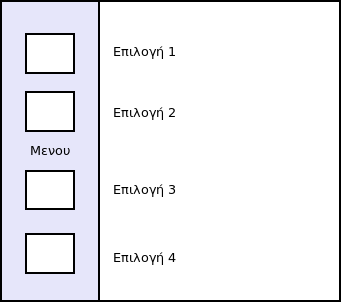
\includegraphics{images/menu.png}}
\caption{Το γενικό μενού (σε αφηρημένη μορφή).}
\label{fig:menu:general}
\end{center}
\end{figure}

\subsubsection{Μενού Παραγγελιών}

\begin{figure}
\begin{center}
\resizebox*{10.5cm}{!}{
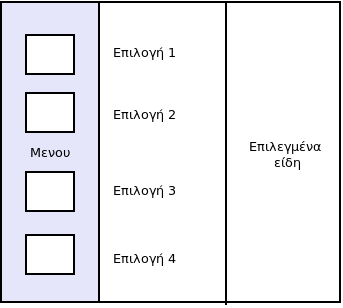
\includegraphics{images/menu_paraggelia.png}}
\caption{Το μενού παραγγελιών (σε αφηρημένη μορφή).}
\label{fig:menu:paraggelia}
\end{center}
\end{figure}

\section{Υλοποίηση και επαλήθευση}

Εδώ να αναφέρουμε για τον κώδικα

\section{Ενσωμάτωση-Τεκμηρίωση}

Ιδέα δεν έχω

\section{Συντήρηση}

Ιδέα δεν έχω

\phantomsection \label{Βιβλιογραφία}
\addcontentsline{toc}{section}{Βιβλιογραφία}
%\mtcaddchapter[Βιβλιογραφία] % Λόγω του minitoc
\bibliographystyle{plain}
\bibliography{references}

\newpage

\end{document}

